\documentclass[lettersize,journal]{IEEEtran}
\usepackage{amsmath,amsfonts}
\usepackage{algorithmic}
\usepackage{algorithm}
\usepackage{array}
\usepackage[caption=false,font=normalsize,labelfont=sf,textfont=sf]{subfig}
\usepackage{textcomp}
\usepackage{stfloats}
\usepackage{url}
\usepackage{verbatim}
\usepackage{graphicx}
\usepackage{cite}
\hyphenation{op-tical net-works semi-conduc-tor IEEE-Xplore}

% ═══════════════════════ PACKAGES ═══════════════════════
\usepackage[T1]{fontenc}
\usepackage[utf8]{inputenc}
\usepackage{amsmath,amssymb,amsfonts}
\usepackage{bm}
\usepackage{graphicx}
\usepackage{cite}
\usepackage{algorithmic}
\usepackage{algorithm}
\usepackage{url}
\usepackage{hyperref}
\usepackage{color}
\usepackage{booktabs}
\usepackage{multirow}
\usepackage{makecell}
%\usepackage{subcaption}  % incompatible with IEEEtran — use subfig instead
\usepackage{siunitx}
\usepackage{pifont}
\usepackage{tikz}
\usepackage{stfloats}
\usetikzlibrary{arrows.meta,positioning,calc}
\usepackage{amsthm}
\newtheorem{proposition}{Proposition}
\renewenvironment{proof}{\noindent\textit{Proof.}}{\hfill$\square$\medskip}

% ═══════════════════════ MATH COMMANDS ═══════════════════
\newcommand{\dq}{\hat{\bm{q}}}
\newcommand{\dqd}{\hat{\bm{q}}_d}
\newcommand{\dqe}{\hat{\bm{q}}_e}
\newcommand{\se}{\mathfrak{se}(3)}
\newcommand{\so}{\mathfrak{so}(3)}
\newcommand{\SE}{SE(3)}
\newcommand{\SO}{SO(3)}
\newcommand{\Spin}{\mathrm{Spin}(3)}
\newcommand{\R}{\mathbb{R}}
\newcommand{\Hd}{\mathbb{H}_d}
\newcommand{\norm}[1]{\left\| #1 \right\|}
\DeclareMathOperator{\Log}{Log}
\DeclareMathOperator{\Exp}{Exp}
\DeclareMathOperator{\Ad}{Ad}
\DeclareMathOperator{\ad}{ad}
\DeclareMathOperator{\atan}{atan2}
\newcommand{\vect}[1]{\bm{#1}}
\newcommand{\mat}[1]{\mathbf{#1}}
\newcommand{\dt}{\Delta t}
\newcommand{\st}{\text{s.t.}}

% Checkmark / cross macros (pifont already loaded)
\newcommand{\cmark}{\textcolor{black}{\ding{51}}}   % ✓
\newcommand{\xmark}{\textcolor{black}{\ding{55}}}   % ✗

% ════════════════════════════════════════════════════════

\begin{document}

\title{Adaptive MPCC via Lie-Invariant MHE for Agile Quadrotor Flight}

\author{Bryan~S.~Guevara,
        Jose~Varela,
        and~Tiago~Nascimento

\thanks{Manuscript received January 14, 2025; revised March 3, 2025.}%
\thanks{Bryan~S.~Guevara is with the Laboratório de Automação
        e Sistemas de Robótica (LaSER), Universidade Federal da
        Paraíba (UFPB), João Pessoa, PB 58051-900, Brazil.
        {\tt\small bguevara@laser.ufpb.br}}%
\thanks{Jose~Varela is with Instituto de Automática (INAUT),
        Universidad Nacional de San Juan--CONICET, Argentina.
        {\tt\small jvarela@inaut.unsj.edu.ar}}%
\thanks{Tiago~Nascimento is with the Laboratório de Automação
        e Sistemas de Robótica (LaSER), Universidade Federal da
        Paraíba (UFPB), João Pessoa, PB 58051-900, Brazil.
        {\tt\small tiago@laser.ufpb.br}}%
\thanks{This work has been supported by the Ministry of Science
        and Innovation of the Spanish Government through the
        research project PID2021-122685OBI00 and the grant
        PRE2019-088069.}%
}

\markboth{IEEE Robotics and Automation Letters}%
{Guevara \MakeLowercase{\textit{et al.}}: Adaptive MPCC via Lie-Invariant MHE for Agile Quadrotor Flight}

\IEEEpubid{0000--0000/00\$00.00~\copyright~2025 IEEE}

\maketitle

\begin{abstract}
Nonlinear Model Predictive Control (NMPC) enables agile quadrotor flight,
yet its performance degrades when the prediction model deviates from the
true plant---a situation that worsens above \SI{8}{m/s} as aerodynamic forces,
mass uncertainty, and actuator lag become simultaneously significant.
No existing approach jointly estimates mass~$m$, body-rate controller
time constant~$\tau_{\mathrm{rc}}$, and a time-varying disturbance
force~$\vect{d}\!\in\!\R^{3}$ online while feeding all three back
into a running NMPC during flight.
We propose a closed-loop architecture coupling a 21-state
Moving Horizon Estimator~(MHE) with a Model Predictive Contouring
Controller~(MPCC).
The MHE employs a Lie-invariant arrival cost on~$\SO$ that is
invariant under the quaternion double cover, eliminating
spurious attitude jumps during hemisphere crossings.
Its posterior covariance drives an adaptive progress
weight~$W_s(k)\!=\!W_{s,\max}/(1\!+\!\alpha\,\sigma_k)$ that
throttles the MPCC while estimates are uncertain and releases it
as they converge---without manual gain scheduling.
In software-in-the-loop experiments at \SI{10}{m/s} on a \SI{100}{m}
Lissajous path with a deliberate 17\,\% mass error, the adaptive
MHE--MPCC reduces position RMSE by 25.9\,\% (from \SI{0.308}{m} to
\SI{0.228}{m}) compared with a fixed-model MPCC baseline, while both
solvers run within a \SI{10}{ms} real-time budget at \SI{100}{Hz}.
\end{abstract}

\begin{IEEEkeywords}
Aerial systems: perception and autonomy,
model predictive control,
moving horizon estimation,
adaptive control,
Lie group methods.
\end{IEEEkeywords}

% ══════════════════════ I. INTRODUCTION ══════════════════
\section{Introduction}
\label{sec:intro}

Quadrotors operating at the limits of their flight envelope demand controllers
that simultaneously handle fast nonlinear dynamics, tight trajectory constraints,
and significant uncertainty in physical parameters.
Nonlinear Model Predictive Control (NMPC) has become the framework of choice
for this regime because it explicitly optimises a receding-horizon cost while
enforcing state and input constraints~\cite{kamel2017linear,falanga2022embedded}.
At low speeds the nominal rigid-body model is sufficiently accurate, but as
flight speed increases beyond 8--10~m/s three categories of mismatch become
critical: (i)~aerodynamic forces that scale with the square of velocity,
(ii)~uncertainty in total vehicle mass $m$ due to changing payloads or
battery state, and (iii)~the finite bandwidth of the low-level body-rate
controller, often modelled as a first-order lag with time constant
$\tau_\mathrm{rc}$.
When the NMPC prediction model ignores these mismatches, planned trajectories
diverge systematically from actual motion, degrading both tracking accuracy
and safety margins.

\subsection*{NMPC and MPCC for Agile UAVs}

NMPC for multirotor vehicles was pioneered by Kamel~\textit{et al.}~\cite{kamel2017linear},
who demonstrated that a full nonlinear formulation outperforms linearised MPC
for aggressive trajectory tracking.
Falanga~\textit{et al.}~\cite{falanga2022embedded} showed that NMPC can be solved onboard
micro aerial vehicles at control frequencies above 50~Hz using tailored
real-time iteration (RTI) schemes.
Building on these foundations, Romero~\textit{et al.}~\cite{romero2022mpcc} introduced
Model Predictive Contouring Control (MPCC), which recasts the tracking problem
as a progress-maximisation problem: a virtual progress variable~$\theta$ traverses
a reference path~$\gamma(\theta)$, and a tuneable weight~$W_s$ on the progress
rate~$\dot\theta$ governs the speed--accuracy trade-off.
MPCC achieves lap times competitive with world-class human pilots.
Krinner~\textit{et al.}~\cite{krinner2024mpccpp} extend MPCC with spatial safety
constraints and a neural-network-learned aerodynamic residual, pushing speeds
beyond 22~m/s.
Yet in both works~$W_s$ is set offline and remains constant throughout flight.
Despite these advances, all NMPC and MPCC formulations to date rely on a
\emph{fixed, nominal} model whose parameters are calibrated offline; any runtime
deviation from the nominal plant is unaccounted for by the prediction model itself.
Moreover, no existing MPCC formulation integrates online parameter or
disturbance estimation of any kind.

\subsection*{Online Disturbance Estimation and Adaptive Strategies}

Three complementary approaches have been proposed to close the gap between model
and reality.

\textit{Adaptive inner-loop augmentation.}
Hanover~\textit{et al.}~\cite{hanover2022performance} cascade an $\mathcal{L}_1$ adaptive controller
around an NMPC outer loop, estimating a lumped matched disturbance $\hat{d}$
at high bandwidth and injecting it as an additive input correction.
The scheme achieves more than 90\% tracking error reduction under unknown payloads
and aggressive manoeuvres up to 20~m/s.
However, the $\mathcal{L}_1$ estimator treats the disturbance as a matched scalar input
channel and does not separately identify physical parameters such as $m$ or
$\tau_\mathrm{rc}$; consequently the NMPC prediction model remains inaccurate
and trajectory optimality cannot be fully recovered.

\textit{Data-driven aerodynamic models.}
Torrente~\textit{et al.}~\cite{torrente2021data} learn an aerodynamic residual force
$\hat{f}_\mathrm{aero}(v)$ with Gaussian Processes trained on offline flight
data, reducing trajectory tracking error by up to 70\% at 14~m/s.
This approach enriches the model fed to NMPC, but the GP is static after training:
it cannot adapt to changes in $m$, to varying $\tau_\mathrm{rc}$ across platforms,
or to time-varying disturbances such as wind gusts.

\textit{Neural and moving-horizon estimators.}
Wang~\textit{et al.}~\cite{wang2024neuromhe} fuse a neural network with a
moving-horizon estimator (NeuroMHE) to estimate the full six-dimensional external
wrench $\hat{w}\in\mathbb{R}^{6}$ and feed it back to the flight controller
in real time, reducing force estimation error by up to 76.7\% over neural
baselines.
A further extension, contextual NeuroMHE~\cite{torshizi2025contextual},
improves generalisation across varying environmental conditions.
Choo and Kayacan~\cite{choo2023data} combine data-driven MHE with Gaussian
Processes for agile quadrotor flight, though hardware validation above 8~m/s
has not been reported.
Critically, none of these estimators isolate the body-rate controller lag
$\tau_\mathrm{rc}$, which introduces systematic phase errors at high angular-rate
commands that cannot be absorbed by an external-force estimate.

\textit{Offline low-level model identification.}
Eschmann~\textit{et al.}~\cite{eschmann2024data} identify motor delay time constants
and inertia parameters via Maximum A Posteriori estimation from one minute of
flight data.
Gupta~\textit{et al.}~\cite{gupta2025lolnmpc} embed identified low-level controller
dynamics, including $\tau_\mathrm{rc}$, directly into the NMPC prediction model,
achieving speeds up to 98~km/h.
Both works perform identification \emph{offline}: $\tau_\mathrm{rc}$ is assumed
constant and is never re-estimated once airborne.
Fan and Copp~\cite{fan2025efficient} propose an online moving-horizon parameter
estimator feeding back structural and thrust parameters to NMPC, but validation
is limited to simulation.

\subsection*{Identified Gap}

\begin{table}[t]
\centering
\caption{%
  Estimation-aware control for agile quadrotors.
  $\hat{m}$\,/\,$\hat{\tau}$ = mass\,/\,body-rate lag estimated online
  (\cmark~online, off = offline, \xmark~no);
  CL = closed-loop correction of prediction model;
  Adp = aggressiveness modulated by estimation confidence.}
\label{tab:comparison}
\setlength{\tabcolsep}{2pt}
\renewcommand{\arraystretch}{1.15}
\footnotesize
\begin{tabular}{@{}lccccccc@{}}
\toprule
\textbf{Work}
  & \textbf{Ctrl}
  & \textbf{$\hat{m}$}
  & \textbf{$\hat{\tau}$}
  & \textbf{Dist.}
  & \textbf{CL}
  & \textbf{Adp}
  & \textbf{\makecell{$v$\\{[m/s]}}} \\
\midrule
\cite{kamel2017linear} Kamel
  & NMPC & \xmark & \xmark & --- & \xmark & \xmark & $<$5 \\
\cite{torrente2021data} Torrente
  & NMPC & \xmark & \xmark & GP$^\dagger$ & $\sim$ & \xmark & 14 \\
\cite{romero2022mpcc} Romero
  & MPCC & \xmark & \xmark & --- & \xmark & \xmark & 16 \\
\cite{krinner2024mpccpp} Krinner
  & MPCC & \xmark & \xmark & NN$^\dagger$ & $\sim$ & \xmark & $>$22 \\
\cite{hanover2022performance} Hanover
  & NMPC & \xmark & \xmark & $\mathcal{L}_1$ & \xmark & \xmark & 20 \\
\cite{wang2024neuromhe} Wang
  & Geom. & \xmark & \xmark & wrench & $\sim$ & \xmark & $<$5 \\
\cite{eschmann2024data} Eschmann
  & NMPC & $\sim$ & off & --- & \xmark & \xmark & $<$5 \\
\cite{gupta2025lolnmpc} Gupta
  & NMPC & \xmark & off & --- & \xmark & \xmark & 27 \\
\cite{fan2025efficient} Fan
  & NMPC & $\sim$ & \xmark & --- & \cmark & \xmark & $<$5$^*$ \\
\cite{zhang2025dual} Zhang
  & NMPC & \xmark & \xmark & MRAC & $\sim$ & \xmark & $<$5 \\
\midrule
\textbf{Ours}
  & \textbf{MPCC} & \cmark & \cmark & \textbf{MHE}
  & \cmark & \cmark & 10 \\
\bottomrule
\end{tabular}

\vspace{2pt}
{\scriptsize $^\dagger$Offline learned.\quad $^*$Simulation only.\quad
Dist.\ column: estimation method for translational disturbance;
all disturbances in acceleration [m/s$^2$] except Wang (wrench [N,\,Nm]).}
\end{table}

As Table~\ref{tab:comparison} summarises, each existing approach addresses
only a subset of the three mismatch sources described above.
Fan and Copp~\cite{fan2025efficient} estimate structural parameters online
via moving-horizon estimation in closed loop with NMPC, but exclude
actuator dynamics and external disturbances, and validate in simulation only.
NeuroMHE~\cite{wang2024neuromhe} estimates the full external wrench online,
yet does not isolate mass or body-rate lag as separate quantities and operates
with a geometric controller at low speeds, not with a predictive controller.
$\mathcal{L}_1$-augmented NMPC~\cite{hanover2022performance} rejects
disturbances at high bandwidth but treats them as a lumped scalar signal,
leaving the prediction model itself uncorrected.
Zhang~\textit{et al.}~\cite{zhang2025dual} cascade dual MRAC channels onto
NMPC to handle payload changes and impacts, but the adaptation is lumped and
does not decompose into separate mass, actuator, and disturbance estimates.
Offline identification~\cite{eschmann2024data,gupta2025lolnmpc} captures
the body-rate lag accurately but cannot track its variation in flight.
Furthermore, all existing MPCC formulations~\cite{romero2022mpcc,krinner2024mpccpp}
use a fixed progress weight tuned offline; the speed--accuracy trade-off
is never adapted to the current estimation confidence.
To the best of our knowledge, the joint online estimation of mass, actuator
lag, and translational disturbance acceleration --- combined with
closed-loop injection into MPCC and confidence-driven progress modulation
--- has not been addressed in the literature.

\subsection*{Contributions}

\begin{enumerate}
    \item An MHE that jointly estimates mass, body-rate lag, and
          translational disturbance acceleration online at 100~Hz,
          using a Lie-invariant arrival cost on the quaternion manifold.

    \item Closed-loop injection of the MHE estimates into the MPCC
          prediction model, correcting mass, actuator dynamics, and
          disturbance at every control step.

    \item An adaptive progress weight driven by the MHE posterior
          covariance, which automatically limits path speed when
          estimates are uncertain and releases it as they converge.

    \item Validation in software-in-the-loop simulation under
          mass mismatch, constant wind, and gust disturbances,
          complemented by hardware experiments on a physical
          quadrotor.
\end{enumerate}

The remainder of this paper is organised as follows.
Section~\ref{sec:model} introduces the quadrotor dynamics and path
parameterisation.
Sections~\ref{sec:mhe} and~\ref{sec:mpcc} formulate the MHE and the
adaptive MPCC, respectively.
Section~\ref{sec:architecture} describes the closed-loop integration.
Section~\ref{sec:results} presents SiL and hardware experiments, and
Section~\ref{sec:conclusion} concludes.

% ══════════════════════ II. SYSTEM MODEL ═════════════════
\section{System Model}
\label{sec:model}

\subsection{Notation}
\label{sec:notation}

Vectors are set in bold italic $\vect{a}$, matrices in bold upright
$\mat{A}$.
The inertial frame is $\mathcal{I}$ and the body frame is
$\mathcal{B}$.
We write $[\vect{a}]_\times\in\R^{3\times3}$ for the skew-symmetric
matrix such that $[\vect{a}]_\times\vect{b}=\vect{a}\times\vect{b}$.
The Hamilton quaternion product is denoted $\otimes$ and is defined so
that $\vect{q}_1\otimes\vect{q}_2$ corresponds to the rotation
$\mat{R}(\vect{q}_1)\mat{R}(\vect{q}_2)$ (composition order).
Unit quaternions are written
$\vect{q}=[q_w,\,\vect{q}_v^\top]^\top\in\mathcal{S}^3\subset\R^4$
with $\norm{\vect{q}}=1$.
The weighted squared norm is
$\norm{\vect{a}}^2_{\mat{W}} \triangleq \vect{a}^\top\mat{W}\,\vect{a}$.

\subsection{Quadrotor Physical Dynamics}

The physical state is
\begin{equation}
  \vect{x}_{\mathrm{phy}}
  = \bigl[\vect{p}^\top,\,\vect{v}^\top,\,\vect{q}^\top,\,
          \vect{\omega}^\top\bigr]^\top
  \in \R^3\!\times\!\R^3\!\times\!\mathcal{S}^3\!\times\!\R^3,
  \label{eq:state_phy}
\end{equation}
where $\vect{p}\in\R^3$ is position in $\mathcal{I}$,
$\vect{v}\in\R^3$ is inertial-frame velocity,
$\vect{q}=[q_w,\vect{q}_v^\top]^\top\in\mathcal{S}^3$ is the unit
quaternion mapping $\mathcal{B}\!\to\!\mathcal{I}$, and
$\vect{\omega}\in\R^3$ is the angular velocity in $\mathcal{B}$.
The continuous-time dynamics are
\begin{subequations}\label{eq:dynamics}
\begin{align}
  \dot{\vect{p}} &= \vect{v}, \label{eq:dp}\\
  \dot{\vect{v}} &= -g\,\vect{e}_3
                    + \frac{f}{m}\,\mat{R}(\vect{q})\,\vect{e}_3
                    + \vect{d}, \label{eq:dv}\\
  \dot{\vect{q}} &= \tfrac{1}{2}\,\vect{q}\otimes
                    [0,\;\vect{\omega}^\top]^\top, \label{eq:dq}\\
  \dot{\vect{\omega}} &= \frac{\vect{\omega}_c - \vect{\omega}}
                              {\tau_{\mathrm{rc}}},
                    \label{eq:domega}
\end{align}
\end{subequations}
where $g=\SI{9.81}{m/s^2}$, $\vect{e}_3=[0,0,1]^\top$, $m$ is the
vehicle mass, $\vect{\omega}_c\in\R^3$ is the body-rate command,
and $\tau_{\mathrm{rc}}>0$ is the first-order time constant of the
low-level rate controller~\cite{gupta2025lolnmpc,eschmann2024data}.
In~\eqref{eq:dv}, $f$ denotes the \emph{thrust state} (not a control
input, see Section~\ref{sec:mpcc_state}), and
$\vect{d}\in\R^3$ is an acceleration disturbance
($\si{m/s^2}$, inertial frame) capturing aerodynamic drag,
payload shifts, and wind.

\noindent\textit{Implementation note.}
In the real-time OCP, equation~\eqref{eq:domega} is equivalently
written as
$\dot{\vect{\omega}} = k_\tau\,(\vect{\omega}_c - \vect{\omega})$
with the \emph{rate gain} $k_\tau \triangleq 1/\tau_{\mathrm{rc}}$
treated as a runtime parameter.
This reparameterisation makes the dynamics \emph{linear} in the
estimated parameter, avoiding the $\mathcal{O}(1/\tau_{\mathrm{rc}}^2)$
Jacobian entries that arise from differentiating $1/\tau_{\mathrm{rc}}$
directly, which would otherwise ill-condition the HPIPM QP solver.
The rotation matrix is
\begin{equation}
  \mat{R}(\vect{q}) = (2q_w^2-1)\,\mat{I}_3
    + 2q_w[\vect{q}_v]_\times + 2\,\vect{q}_v\vect{q}_v^\top,
  \label{eq:R_from_q}
\end{equation}
which implements the \emph{active} body-to-inertial rotation under
the Hamilton convention.

\subsection{Path Parameterisation}
\label{sec:path}

A 3-D Lissajous figure is parameterised in arc-length $\theta$
via offline B-spline fitting to $N_{\mathrm{wp}}=400$ waypoints
sampled from the time-parametric trajectory
at $s_{\max}=\SI{100}{m}$~\cite{romero2022mpcc}.
The B-spline map
\begin{equation}
  \gamma(\theta)
  = \bigl[\vect{p}_d(\theta),\;\vect{q}_d(\theta),\;
          \hat{\vect{\omega}}(\theta)\bigr]
  \label{eq:bspline}
\end{equation}
yields: path position $\vect{p}_d\in\R^3$, attitude reference
$\vect{q}_d\in\mathcal{S}^3$ (from differential flatness~\cite{falanga2022embedded},
max tilt \SI{60}{\degree}), and the unit tangent
$\vect{\tau}(\theta)=\partial\vect{p}_d/\partial\theta/
\norm{\partial\vect{p}_d/\partial\theta}$.
A feedforward thrust could be derived from the path via differential
flatness, but is unnecessary here because thrust is a state governed
by the rate input $\Delta f$.
The angular-velocity sensitivity
$\hat{\vect{\omega}}(\theta)\in\R^3$ is the body-frame angular rate
per unit arc-length,
$\hat{\vect{\omega}} = 2\bigl(\vect{q}_d^*\otimes
\mathrm{d}\vect{q}_d/\mathrm{d}\theta\bigr)\!\big|_{\mathrm{vec}}$.
The angular-velocity feedforward then scales with progress speed:
\begin{equation}
  \vect{\omega}_d(\theta,v_\theta) = \hat{\vect{\omega}}(\theta)\,v_\theta.
  \label{eq:omega_ff}
\end{equation}

% ══════════════════════ III. LIE-INVARIANT MHE ═══════════
\section{Lie-Invariant Moving Horizon Estimator}
\label{sec:mhe}

\subsection{Augmented State for Online Estimation}

The uncertain parameters $m$, $\tau_{\mathrm{rc}}$, and $\vect{d}$
are treated as slowly varying states.
Together with the physical state~\eqref{eq:state_phy} and the MPCC
virtual states $(\theta,v_\theta,f)$ introduced in
Section~\ref{sec:mpcc_state}, the MHE augmented state is
\begin{equation}
  \vect{x}_a = \bigl[\vect{x}_{\mathrm{phy}}^\top,\,
                \theta,\,v_\theta,\,f,\,
                m,\, \tau_{\mathrm{rc}},\,
                \vect{d}^\top\bigr]^\top \in \R^{21},
  \label{eq:augmented_state}
\end{equation}
with random-walk drift dynamics
\begin{equation}
  \dot{m} = w_m,\quad
  \dot{\tau}_{\mathrm{rc}} = w_\tau,\quad
  \dot{\vect{d}} = \vect{w}_d,
  \label{eq:param_dynamics}
\end{equation}
where $\vect{w}_a=[w_m,\,w_\tau,\,\vect{w}_d^\top]^\top\in\R^5\sim
\mathcal{N}(\vect{0},\mat{Q}_w)$.

\subsection{Measurement Model}

The odometry system provides $\vect{x}_{\mathrm{phy}}$ at discrete
times $t_k=k\dt$.
Because the quaternion lives on $\mathcal{S}^3$, the measurement
function is \emph{nonlinear}:
\begin{equation}
  \vect{y}_k = h\!\bigl(\vect{x}_{a,k}\bigr) + \vect{n}_k,\quad
  \vect{n}_k\sim\mathcal{N}(\vect{0},\mat{R}_n),
  \label{eq:measurement}
\end{equation}
where the residual $\vect{r}_k = \vect{y}_k - h(\vect{x}_{a,k}) \in\R^{12}$
is computed using the same Lie-invariant Log map as the arrival cost
(Section~\ref{sec:arrival}):
\begin{equation}
  h(\vect{x}_a)
  = \bigl[\vect{p}^\top,\;\vect{v}^\top,\;
          \vect{\varepsilon}_q(\vect{q},\vect{y}_{q})^\top,\;
          \vect{\omega}^\top\bigr]^\top,
  \label{eq:h_meas}
\end{equation}
so the measurement cost becomes
$\ell_y = \norm{\vect{r}_k}^2_{\mat{R}_n^{-1}}$ with
$\mat{R}_n = \mathrm{diag}(\sigma_p^2\mat{I}_3,\,
             \sigma_v^2\mat{I}_3,\,\sigma_q^2\mat{I}_3,\,
             \sigma_\omega^2\mat{I}_3)\in\R^{12\times12}$.
The quaternion block contributes a 3-dimensional tangent-space residual
rather than the 4-dimensional raw difference.
The parameters $(m,\tau_{\mathrm{rc}},\vect{d})$ are not directly measured;
they are identified through prediction residuals in the
dynamics~\eqref{eq:dynamics}.

\subsection{MHE Optimal Control Problem}

At time step $k$ the MHE estimates the augmented state trajectory
over the past $N_e$ steps.
Let $\bar{\vect{x}}_{a}$ and $\bar{\mat{P}}$ denote the prior mean
and covariance at the window start $k\!-\!N_e$.
The estimator solves
\begin{subequations}\label{eq:mhe_ocp}
\begin{align}
  \min_{\substack{\vect{x}_{a,j},\;\vect{w}_{a,j}\\j\in[k-N_e,\,k]}}
  \;\;& \Phi_{\mathrm{arr}}\!\bigl(\vect{x}_{a,k-N_e}\bigr)
  + \sum_{j=k-N_e}^{k-1}\!
    \Bigl[\ell_y\!\bigl(\vect{y}_j,\vect{x}_{a,j}\bigr)
    + \norm{\vect{w}_{a,j}}^2_{\mat{Q}_w^{-1}}\Bigr]
  + \ell_y\!\bigl(\vect{y}_k,\vect{x}_{a,k}\bigr)
  \label{eq:mhe_cost}\\
  \st\quad
  & \vect{x}_{a,j+1} = F\!\bigl(\vect{x}_{a,j},\,\vect{u}_j\bigr)
                       + \mat{G}\,\vect{w}_{a,j},
  \label{eq:mhe_dyn}\\
  & \vect{x}_{a,j} \in \mathcal{X}_a,
  \label{eq:mhe_bounds}
\end{align}
\end{subequations}
where $F:\R^{21}\!\times\!\R^5\!\to\!\R^{21}$ is the discretised
augmented dynamics~\eqref{eq:dynamics}--\eqref{eq:param_dynamics},
$\mat{G}\in\R^{21\times5}$ maps process noise into the five
parameter slots $[m,\tau_{\mathrm{rc}},\vect{d}^\top]^\top$, and
$\mathcal{X}_a$ enforces physical bounds on the estimated
parameters and states (see Table~\ref{tab:solver_params}).
The measurement cost uses the Lie-invariant residual~\eqref{eq:h_meas}:
\begin{equation}
  \ell_y(\vect{y}_j,\vect{x}_{a,j})
  = \norm{\vect{y}_j - h(\vect{x}_{a,j})}^2_{\mat{R}_n^{-1}}.
  \label{eq:meas_cost}
\end{equation}

\subsection{Lie-Invariant Arrival Cost}
\label{sec:arrival}

The arrival cost $\Phi_{\mathrm{arr}}$ summarises information
accumulated before the current window.
A Euclidean formulation,
\begin{equation}
  \Phi_{\mathrm{arr}}^{\text{Eucl}}(\vect{x}_a)
  = \norm{\vect{x}_a - \bar{\vect{x}}_{a}}^2_{\bar{\mat{P}}^{-1}},
  \label{eq:euclidean_arrival}
\end{equation}
treats quaternions as elements of $\R^4$.
Because both $\vect{q}$ and $-\vect{q}$ represent the same
rotation in $\SO$, this cost is \emph{not} invariant under the
double-cover map $\pi:\mathcal{S}^3\to\SO$:
when the estimator state crosses a hemisphere boundary,
$\norm{\vect{q}-\bar{\vect{q}}}^2$ reports a spurious error
even though $\mat{R}(\vect{q})=\mat{R}(\bar{\vect{q}})$.

We replace the quaternion block with the left-invariant Riemannian
metric on $\SO$.
Define the quaternion error
\begin{equation}
  \vect{q}_e = \bar{\vect{q}}^{-1}\otimes\vect{q},\qquad
  \bar{\vect{q}}^{-1}\triangleq[\bar{q}_w,\,-\bar{\vect{q}}_v^\top]^\top,
  \label{eq:q_error}
\end{equation}
and apply the hemisphere correction
\begin{equation}
  \tilde{\vect{q}}_e = \operatorname{sgn}(q_{e,w})\,\vect{q}_e
  \label{eq:hemisphere}
\end{equation}
to ensure $\tilde{q}_{e,w}\ge0$, where
$\operatorname{sgn}(0)\triangleq 1$.
The rotation-vector error in $\so\cong\R^3$ is
\begin{equation}
  \vect{\varepsilon}_q(\vect{q},\bar{\vect{q}})
  = \Log_{\mathcal{S}^3}\!\bigl(\tilde{\vect{q}}_e\bigr)
  \triangleq 2\,\frac{\atan\!\bigl(\norm{\tilde{\vect{q}}_{e,v}},\,
                     \tilde{q}_{e,w}\bigr)}
             {\norm{\tilde{\vect{q}}_{e,v}}+\epsilon}\,
    \tilde{\vect{q}}_{e,v},
  \label{eq:log_map}
\end{equation}
with $\epsilon=10^{-9}$ for numerical stability.
The factor of 2 arises because the unit quaternion encodes
the half-angle: $\vect{q}=[\cos(\phi/2),\,\sin(\phi/2)\,\vect{n}^\top]^\top$
for rotation angle $\phi$ about axis $\vect{n}$, so the standard
$\SO$ logarithm $\Log_{\SO(3)}(\mat{R})=\phi\,\vect{n}$ requires
$\phi = 2\arctan(\norm{\vect{q}_v},q_w)$.

The Lie-invariant arrival cost is
\begin{multline}
  \Phi_{\mathrm{arr}}(\vect{x}_a)
  = \norm{\vect{p}-\bar{\vect{p}}}^2_{\mat{P}_p^{-1}}
  + \norm{\vect{v}-\bar{\vect{v}}}^2_{\mat{P}_v^{-1}}
  + \norm{\vect{\varepsilon}_q}^2_{\mat{P}_q^{-1}} \\
  + \norm{\vect{\omega}-\bar{\vect{\omega}}}^2_{\mat{P}_\omega^{-1}}
  + \norm{\vect{\theta}-\bar{\vect{\theta}}}^2_{\mat{P}_\theta^{-1}},
  \label{eq:lie_arrival}
\end{multline}
where
$\vect{\theta}\triangleq[m,\,\tau_{\mathrm{rc}},\,\vect{d}^\top]^\top
\!\in\!\R^5$
collects the estimated parameters,
$\mat{P}_{(\cdot)}\succ 0$ are the corresponding diagonal blocks of
$\bar{\mat{P}}$, and the virtual-state block
$\mat{P}_{\xi}\in\R^{3\times3}$ covers
$(\theta,v_\theta,f)$.
The quaternion block $\mat{P}_q\in\R^{3\times3}$ operates in the
tangent space $\so\cong\R^3$, not $\R^4$, so $\bar{\mat{P}}$ is
$20\times20$ rather than $21\times21$.

The hemisphere correction~\eqref{eq:hemisphere} ensures that the
arrival cost~\eqref{eq:lie_arrival} is invariant under the
double-cover sign flip $\vect{q}\mapsto-\vect{q}$: flipping the
sign of $\vect{q}$ negates the error quaternion $\vect{q}_e$, but
the $\operatorname{sgn}(\cdot)$ factor absorbs the extra minus sign,
leaving $\tilde{\vect{q}}_e$ and therefore $\Phi_{\mathrm{arr}}$
unchanged.
This prevents fictitious attitude jumps when the quaternion crosses
the $q_w\!=\!0$ hemisphere boundary during aggressive
manoeuvres --- precisely the regime encountered at peak-curvature
points of the Lissajous trajectory (Section~\ref{sec:results}).

\subsection{Arrival Cost Propagation}

After each solved window, the prior is propagated by one step using
an extended Kalman prediction:
\begin{subequations}\label{eq:arrival_prop}
\begin{align}
  \bar{\vect{x}}_{a}^+ &= F\!\bigl(\hat{\vect{x}}_{a,k-N_e},\,
                           \vect{u}_{k-N_e}\bigr),
  \label{eq:prior_mean}\\
  \bar{\mat{P}}^+ &= \mat{A}_k\,\bar{\mat{P}}\,\mat{A}_k^\top
                     + \mat{G}\,\mat{Q}_w\,\mat{G}^\top,
  \label{eq:prior_cov}
\end{align}
\end{subequations}
where
$\mat{A}_k=\partial F/\partial\vect{x}_a\big|_{\hat{\vect{x}}_{a,k-N_e}}$
is the discrete-dynamics Jacobian and $\hat{\vect{x}}_{a,k-N_e}$ is
the MHE solution at the oldest node.
The Jacobian $\mat{A}_k$ is $20\!\times\!20$ because the quaternion
block is evaluated in the $\R^3$ tangent space via
$\delta\vect{q}\approx\frac{1}{2}\vect{q}\otimes[0,\,\delta\vect{\phi}^\top]^\top$,
consistent with the Log map~\eqref{eq:log_map}.


% ══════════════════════ IV. ADAPTIVE MPCC ════════════════
\section{Adaptive Model Predictive Contouring Control}
\label{sec:mpcc}

Given the parameter estimates $\hat{\vect{\theta}}_k$ and uncertainty
$\sigma_k$ from the MHE (Section~\ref{sec:mhe}), we now formulate
the MPCC that consumes these outputs to adapt its prediction model
and aggressiveness online.

\subsection{MPCC Virtual States and Control Input}
\label{sec:mpcc_state}

Model Predictive Contouring Control appends three virtual states
to track path progress~\cite{romero2022mpcc}:
arc-length $\theta\in\R_{\ge0}$ [m],
progress velocity $v_\theta\in\R_{\ge0}$ [m/s],
and collective thrust $f\in\R_{\ge0}$ [N].
The \emph{thrust-as-state} formulation~\cite{romero2022mpcc} avoids
discontinuous thrust commands: the control input is the thrust
\emph{rate} $\Delta f = \dot{f}$, so $f$ evolves smoothly.
The full MPCC state and control vectors are
\begin{equation}
  \vect{x} = [\vect{x}_{\mathrm{phy}}^\top,\;\theta,\;v_\theta,\;f]^\top
             \in\R^{16},\qquad
  \vect{u} = [\Delta f,\;\vect{\omega}_c^\top,\;a_\theta]^\top\in\R^5,
  \label{eq:mpcc_state}
\end{equation}
where $a_\theta = \dot{v}_\theta$ is the progress acceleration.
The virtual-state dynamics extend~\eqref{eq:dynamics} with
\begin{equation}
  \dot{\theta} = v_\theta,\qquad
  \dot{v}_\theta = a_\theta,\qquad
  \dot{f} = \Delta f.
  \label{eq:virtual_dyn}
\end{equation}
All 16 states are integrated inside the OCP via ERK4; only the
physical states $\vect{x}_{\mathrm{phy}}$ are fed back from odometry
at runtime (Section~\ref{sec:architecture}).

\subsection{Contouring and Lag Error Decomposition}
\label{sec:errors}

At arc-length $\theta$, the position error to the path is
$\vect{e}_t(\theta) = \vect{p}_d(\theta) - \vect{p}$.
This decomposes orthogonally into:
\begin{subequations}\label{eq:errors}
\begin{align}
  e_l(\theta) &= \vect{\tau}(\theta)^\top\vect{e}_t(\theta), \label{eq:lag}\\
  \vect{e}_c(\theta) &= \mat{P}_\perp(\theta)\,\vect{e}_t(\theta),\label{eq:cont}
\end{align}
\end{subequations}
where $\mat{P}_\perp(\theta)=\mat{I}_3-\vect{\tau}\vect{\tau}^\top$
is the contouring projector.
The decomposition satisfies
$\norm{\vect{e}_t}^2 = e_l^2 + \norm{\vect{e}_c}^2$.

\subsection{Contouring Cost and Lie-Invariant Attitude Error}

At prediction stage $j\in\{0,\ldots,N\}$, with path parameter
$\theta_j$ and drone attitude $\vect{q}_j$, the attitude error is
computed via the same Log map used in Section~\ref{sec:arrival},
evaluated at the path-referenced attitude $\vect{q}_d(\theta_j)$:
\begin{equation}
  \vect{\varepsilon}_{q,j}
  = \Log_{\mathcal{S}^3}\!\bigl(\tilde{\vect{q}}_{e,j}\bigr),\quad
  \vect{q}_{e,j} = \vect{q}_d(\theta_j)^{-1}\otimes\vect{q}_j,
  \label{eq:att_err_mpcc}
\end{equation}
with hemisphere correction~\eqref{eq:hemisphere}.
Using the same geometric error in both the MHE arrival cost and the
MPCC stage cost ensures end-to-end Lie-invariant consistency.

The angular-rate tracking error with feedforward~\eqref{eq:omega_ff}
is
\begin{equation}
  \tilde{\vect{\omega}}_j
  = \vect{\omega}_{c,j} - \hat{\vect{\omega}}(\theta_j)\,v_{\theta,j}
  \in\R^3.
  \label{eq:rate_err}
\end{equation}

The stage cost is
\begin{multline}
  \ell(\vect{x}_j,\vect{u}_j)
  = \norm{\vect{e}_{c,j}}^2_{\mat{Q}_c}
  + e_{l,j}^2\,Q_l
  + \norm{\vect{\varepsilon}_{q,j}}^2_{\mat{Q}_q} \\
  + W_{\Delta f}\,\Delta f_j^2
  + \norm{\tilde{\vect{\omega}}_j}^2_{\mat{W}_\omega}
  - W_s(k)\,v_{\theta,j},
  \label{eq:mpcc_stage}
\end{multline}
and the terminal cost (no progress term) is
\begin{equation}
  \ell_N(\vect{x}_N)
  = \norm{\vect{e}_{c,N}}^2_{\mat{Q}_c}
  + e_{l,N}^2\,Q_l
  + \norm{\vect{\varepsilon}_{q,N}}^2_{\mat{Q}_q}.
  \label{eq:mpcc_terminal}
\end{equation}
The negative term $-W_s(k)\,v_{\theta,j}$ maximises progress speed
along the path; all other terms penalise deviations.
The weight matrices $\mat{Q}_c,Q_l,\mat{Q}_q,\mat{W}_\omega\succ0$
and scalar $W_{\Delta f}>0$ are fixed; only $W_s(k)$ varies online.

\subsection{MPCC Optimal Control Problem}

At step $k$ the MPCC solves the OCP over the
\emph{16-state} model~\eqref{eq:mpcc_state}--\eqref{eq:virtual_dyn}:
\begin{subequations}\label{eq:mpcc_ocp}
\begin{align}
  \min_{\vect{u}_0,\ldots,\vect{u}_{N-1}}
  \;&
  \sum_{j=0}^{N-1}\!\ell(\vect{x}_j,\vect{u}_j) + \ell_N(\vect{x}_N)
  \label{eq:mpcc_obj}\\
  \st\quad
  & \vect{x}_0 = \hat{\vect{x}}_k,
  \label{eq:mpcc_ic}\\
  & \vect{x}_{j+1} = F\!\bigl(\vect{x}_j,\vect{u}_j;\,
    \hat{m}_k,\,\hat{k}_{\tau,k},\,\hat{\vect{d}}_k\bigr),
  \label{eq:mpcc_dyn}\\
  & 0\!\le\! f_j\!\le\!T_{\max},\;
    |\Delta f_j|\!\le\!\Delta f_{\max},
  \label{eq:thrust_bounds}\\
  & \norm{\vect{\omega}_{c,j}}_\infty\!\le\!\omega_{\max},\;
    0\!\le\! v_{\theta,j}\!\le\! v_{\theta,\max},
  \label{eq:rate_bounds}\\
  & |e_{l,j}|\le D_{\max}\quad\text{(soft, L2 penalty)}.
  \label{eq:lag_soft}
\end{align}
\end{subequations}
The dynamics $F$ in~\eqref{eq:mpcc_dyn} integrate the full 16-state
model using the MHE parameter estimates
$\hat{\vect{\theta}}_k=[\hat{m}_k,\,\hat{k}_{\tau,k},\,
\hat{\vect{d}}_k^\top]^\top\in\R^5$
as fixed runtime parameters within the prediction horizon, where
$\hat{k}_{\tau,k}=1/\hat{\tau}_{\mathrm{rc},k}$ (see implementation
note in Section~\ref{sec:model}).
To prevent premature injection of unconverged estimates, the parameter
update is gated: only when $\sigma_k < \sigma_{\mathrm{thr}}$ does the
MPCC receive $\hat{\vect{\theta}}_k$; otherwise it falls back to
nominal values $\vect{\theta}_0=[m_0,\,k_{\tau,0},\,\vect{0}]^\top$.
Furthermore, an \emph{exponential moving average} (EMA) is applied
to the raw MHE output before injection, suppressing window-shift
step changes without introducing estimator bias.
Constraint~\eqref{eq:lag_soft} prevents excessive lag accumulation.
All design parameters are listed in Table~\ref{tab:solver_params}
(Section~\ref{sec:setup}).

\subsection{Adaptive Progress Weight}
\label{sec:adaptive_ws}

The scalar $\sigma_k = \operatorname{tr}(\bar{\mat{P}}_{\theta,k})$,
where $\bar{\mat{P}}_{\theta,k}\in\R^{5\times5}$ is the parameter
uncertainty block of the MHE prior covariance at step $k$, quantifies
how well $\hat{\vect{\theta}}_k$ is currently known.
We define the \emph{adaptive progress weight}
\begin{equation}
  W_s(k) = \frac{W_{s,\max}}{1 + \alpha\,\sigma_k},
  \label{eq:adaptive_ws}
\end{equation}
where $W_{s,\max}>0$ sets the maximum aggressiveness and $\alpha>0$
controls sensitivity.

\noindent\textbf{Physical interpretation.}
When $\sigma_k$ is large (estimator uncertain, e.g.\ unknown payload
just attached), $W_s(k)\!\to\!0$ and the MPCC does not push $v_\theta$
hard — it tracks the path conservatively while the MHE gathers
information.
As $\hat{m}_k$ and $\hat{\vect{d}}_k$ converge, $\sigma_k$ decreases
and $W_s(k)\!\to\!W_{s,\max}$: the controller progressively recovers
near-optimal lap time with no manual intervention.

\noindent\textbf{Implementation.}
$W_s(k)$ is computed outside the OCP and injected as runtime parameter
$p[13]$ via the acados parameter interface at each control step.
This requires no structural change to the OCP — only a scalar update
costs negligible computation.


% ══════════════════════ V. ARCHITECTURE ══════════════════
\section{Closed-Loop Architecture}
\label{sec:architecture}

\begin{figure}[t]
\centering
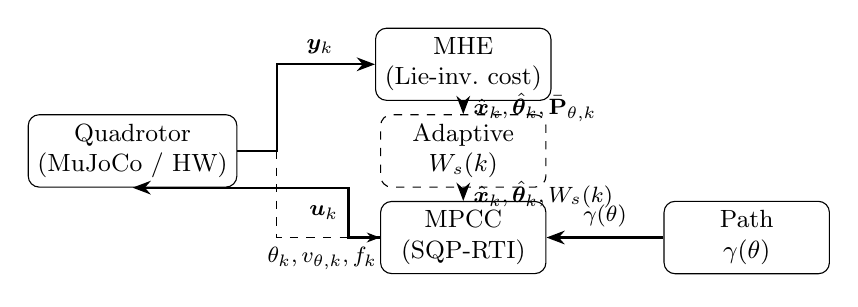
\begin{tikzpicture}[
    block/.style={draw, rounded corners, minimum width=2.1cm,
                  minimum height=0.8cm, align=center, font=\small},
    adapt/.style={draw, rounded corners, minimum width=2.1cm,
                  minimum height=0.7cm, align=center, font=\small,
                  dashed},
    arrow/.style={-Stealth, thick},
    every node/.style={font=\small}
  ]
  % Nodes
  \node[block] (plant) at (0,   0)    {Quadrotor\\(MuJoCo / HW)};
  \node[block] (mhe)   at (4.2, 1.1)  {MHE\\(Lie-inv.\ cost)};
  \node[adapt] (adapt) at (4.2, 0)    {Adaptive\\$W_s(k)$};
  \node[block] (mpcc)  at (4.2,-1.1)  {MPCC\\(SQP-RTI)};
  \node[block] (path)  at (7.8,-1.1)  {Path\\$\gamma(\theta)$};

  % Plant → MHE (measurement)
  \draw[arrow] (plant.east) -- ++(0.5,0)
               coordinate (fork) |- (mhe.west)
               node[above, pos=0.72]{\footnotesize$\vect{y}_k$};

  % Plant → MPCC (virtual states, thin dashed)
  \draw[arrow, dashed, thin] (fork) |- (mpcc.west)
               node[below, pos=0.72]
               {\footnotesize$\theta_k,v_{\theta,k},f_k$};

  % MHE → adapt block
  \draw[arrow] (mhe.south) --
               node[right]{\footnotesize$\hat{\vect{x}}_k,\hat{\vect{\theta}}_k,\bar{\mat{P}}_{\theta,k}$}
               (adapt.north);

  % adapt → MPCC
  \draw[arrow] (adapt.south) --
               node[right]{\footnotesize$\hat{\vect{x}}_k,\hat{\vect{\theta}}_k,W_s(k)$}
               (mpcc.north);

  % Path → MPCC
  \draw[arrow] (path.west) --
               node[above]{\footnotesize$\gamma(\theta)$}
               (mpcc.east);

  % MPCC → plant
  \draw[arrow] (mpcc.west) -- ++(-0.4,0) |-
               node[left, pos=0.25]{\footnotesize$\vect{u}_k$}
               (plant.south);
\end{tikzpicture}
\caption{Closed-loop MHE--MPCC architecture.
  The MHE accumulates $N_e\!=\!20$ past measurements and returns:
  physical state estimate $\hat{\vect{x}}_k\!\in\!\R^{13}$,
  parameter estimate $\hat{\vect{\theta}}_k\!=\![\hat{m}_k,\,\hat{k}_{\tau,k},\,
  \hat{\vect{d}}_k^\top]^\top\!\in\!\R^5$ (where $\hat{k}_{\tau}=1/\hat{\tau}_{\mathrm{rc}}$), and
  prior covariance block $\bar{\mat{P}}_{\theta,k}\!\in\!\R^{5\times5}$.
  The adaptive block computes $\sigma_k\!=\!\operatorname{tr}(\bar{\mat{P}}_{\theta,k})$
  and injects $W_s(k)$ as a runtime parameter into the MPCC.
  Virtual states $(\theta_k,v_{\theta,k},f_k)$ are integrated
  outside the solver and fed forward to the MPCC initial condition.
  Both solvers run sequentially at \SI{100}{\hertz}.}
\label{fig:architecture}
\end{figure}

Algorithm~\ref{alg:main} summarises the online loop.
The MHE and MPCC share no internal solver state; their coupling is
one-directional: the MHE output $(\hat{\vect{x}}_k,\hat{\vect{\theta}}_k)$
is injected into the MPCC as initial condition and model parameters.
The additional signal $\bar{\mat{P}}_{\theta,k}$ feeds the adaptive
weight~\eqref{eq:adaptive_ws} without altering the OCP structure.
At step~3, the MHE solution $\hat{\vect{x}}_{a,k}\!\in\!\R^{21}$ is
decomposed as: physical states
$\hat{\vect{x}}_k\!=\!\hat{\vect{x}}_{a,k}[1\!:\!13]$,
virtual states
$(\hat{\theta}_k,\hat{v}_{\theta,k},\hat{f}_k)\!=\!\hat{\vect{x}}_{a,k}[14\!:\!16]$,
and parameters
$\hat{\vect{\theta}}_k\!=\![\hat{m}_k,\hat{\tau}_{\mathrm{rc},k},
\hat{\vect{d}}_k^\top]^\top
=\hat{\vect{x}}_{a,k}[17\!:\!21]$,
from which $\hat{k}_{\tau,k}=1/\hat{\tau}_{\mathrm{rc},k}$
is computed before injection into the MPCC.

\begin{algorithm}[t]
\caption{Online MHE--MPCC control loop (\SI{100}{\hertz})}
\label{alg:main}
\begin{algorithmic}[1]
\REQUIRE Prior $(\bar{\vect{x}}_a,\,\bar{\mat{P}})$;
         precomputed path $\gamma(\theta)$;
         virtual states $(\theta_0,v_{\theta,0},f_0)$.
\FOR{$k = 0, 1, 2, \ldots$}
  \STATE Read odometry $\vect{y}_k$
  \STATE \textbf{MHE}: solve~\eqref{eq:mhe_ocp}
         $\;\Rightarrow\;
         \hat{\vect{x}}_k\!\in\!\R^{13},\;
         \hat{\vect{\theta}}_k\!\in\!\R^5,\;
         \bar{\mat{P}}_{\theta,k}\!\in\!\R^{5\times5}$
  \STATE Propagate arrival cost prior:
         $(\bar{\vect{x}}_a^+,\bar{\mat{P}}^+)$
         via~\eqref{eq:arrival_prop}
  \STATE Compute uncertainty and adaptive weight:
         $\sigma_k \gets \operatorname{tr}(\bar{\mat{P}}_{\theta,k})$,\;
         $W_s(k) \gets W_{s,\max}/(1+\alpha\,\sigma_k)$
  \STATE Apply EMA filter to raw MHE output:
         $\hat{\vect{\theta}}_k^{\mathrm{ema}} \gets
           \vect{\alpha}\!\odot\!\hat{\vect{\theta}}_{k-1}^{\mathrm{ema}}
           + (\vect{1}-\vect{\alpha})\!\odot\!\hat{\vect{\theta}}_k$
  \STATE Determine injected parameters:
         $\hat{\vect{\theta}}_k^{\mathrm{inj}} \gets
           \hat{\vect{\theta}}_k^{\mathrm{ema}}$
         if $\sigma_k < \sigma_{\mathrm{thr}}$,
         else $\vect{\theta}_0$ (nominal)
  \STATE \textbf{MPCC}: set initial condition
         $\vect{x}_0\!=\![\hat{\vect{x}}_k^\top,\,\theta_k,\,v_{\theta,k},\,f_k]^\top$,
         update $\hat{\vect{\theta}}_k^{\mathrm{inj}}$ in~\eqref{eq:mpcc_dyn},
         inject $W_s(k)$ as runtime parameter;\\
         \quad solve~\eqref{eq:mpcc_ocp}
         $\;\Rightarrow\;
         \vect{u}_k^*=[\Delta f_k^*,\,\vect{\omega}_{c,k}^{*\top},\,a_{\theta,k}^*]^\top$
  \STATE Integrate virtual states (Euler):
         $\theta_{k+1}\!\gets\!\theta_k + v_{\theta,k}\,\Delta t$;\;
         $v_{\theta,k+1}\!\gets\!v_{\theta,k} + a_{\theta,k}^*\,\Delta t$;\;
         $f_{k+1}\!\gets\!f_k + \Delta f_k^*\,\Delta t$
  \STATE Apply commands: thrust $f_k$, body rates $\vect{\omega}_{c,k}^*$
\ENDFOR
\end{algorithmic}
\end{algorithm}

% ══════════════════════ VI. RESULTS ════════════════════════
\section{Experimental Results}
\label{sec:results}

This section validates the closed-loop MHE--MPCC architecture
(Algorithm~\ref{alg:main}) in three stages: (i)~SiL experiments
with mass mismatch, (ii)~SiL experiments with wind disturbances,
and (iii)~hardware experiments on a physical quadrotor.

\subsection{Experimental Setup}
\label{sec:setup}

\subsubsection{Platform}
The SiL experiments use MuJoCo with full rigid-body contact dynamics
and a realistic motor model, interfaced via ROS\,2 Humble at
\SI{100}{\hertz} ($\Delta t=\SI{10}{ms}$).
Hardware experiments use the same software stack deployed on
a custom quadrotor with onboard state estimation.
Both solvers are generated with
acados~\cite{verschueren2022acados}/CasADi~\cite{andersson2019casadi}
and execute single-threaded on an Intel Core~i7.
Table~\ref{tab:solver_params} lists all design parameters.

\begin{table}[t]
\centering
\caption{MPCC and MHE design parameters.}
\label{tab:solver_params}
\setlength{\tabcolsep}{4pt}
\begin{tabular}{@{}lcc@{}}
\toprule
\textbf{Parameter} & \textbf{MPCC} & \textbf{MHE} \\
\midrule
States / controls      & $16$ / $5$       & $21$ (aug.) / $5$     \\
Horizon stages $N$     & $50$             & $N_e=20$        \\
Time grid $T_h$        & \SI{1.5}{s} (non-unif.) & \SI{0.2}{s} \\
Integrator             & ERK4             & ERK4            \\
QP solver              & HPIPM            & HPIPM           \\
NLP solver             & SQP-RTI (1 iter) & SQP-RTI (1 iter)\\
Regularisation         & PROJECT + LM     & PROJECT\_REDUC + LM \\
$m$ bounds             & —                & $[0.5,\;\SI{3.0}{kg}]$ \\
$\tau_{\mathrm{rc}}$ bounds & —           & $[0.005,\;\SI{0.15}{s}]$ \\
$\norm{\vect{d}}_\infty$ bound & —       & $\SI{8}{m/s^2}$ \\
$f$ bounds             & $[0,\;\SI{49.05}{N}]$ & —          \\
$\Delta f_{\max}$      & \SI{500}{N/s}    & —               \\
$\omega_{\max}$        & \SI{20}{rad/s}   & —               \\
$a_{\theta}$ bounds    & $\pm 4g$\;\si{m/s^2} & —           \\
$v_{\theta,\max}$      & \SI{14}{m/s}     & —               \\
$D_{\max}$ (lag)       & \SI{0.5}{m}      & —               \\
$\sigma_{\mathrm{thr}}$ & $0.05$          & —               \\
$\alpha_{\mathrm{EMA},m/\tau}$ & $0.98$  & —               \\
$\alpha_{\mathrm{EMA},d}$ & $0.92$       & —               \\
\bottomrule
\end{tabular}
\end{table}

\subsubsection{Path and speed}
The reference path is a three-dimensional Lissajous figure
parameterised in arc-length with $s_{\max}=\SI{100}{m}$
(Section~\ref{sec:path}), traversed at a maximum progress speed
$v_{\theta,\max}=\SI{10}{m/s}$.

\subsubsection{Mass mismatch scenario}
A deliberate mass error is introduced: the true vehicle mass is
$m_{\mathrm{true}}=\SI{1.08}{kg}$ while both modes are initialised
with a nominal guess $m_0=\SI{0.9}{kg}$, corresponding to a
$-17\%$ error.

\subsubsection{Wind disturbance scenarios}
Three wind profiles are applied via MuJoCo's external force interface
to evaluate the disturbance estimator $\hat{\vect{d}}$:
\begin{itemize}
  \item \textbf{Constant wind:} a steady force
        ($\approx$10\% of vehicle weight) along the inertial
        $x$-axis throughout the flight.
  \item \textbf{Gust:} a short-duration impulse applied at
        mid-flight, simulating a localised wind burst.
  \item \textbf{Turbulence:} band-limited random forcing with
        a Dryden-like spectrum, applied on all three axes.
\end{itemize}

\subsubsection{Compared modes}
Two operating modes are compared:
\begin{itemize}
  \item \textbf{v1 (open-loop baseline):} The MHE runs but the
        injection gate is permanently disabled; the MPCC uses fixed
        nominal parameters
        $\vect{\theta}_0=[m_0,\,k_{\tau,0},\,\vect{0}]^\top$.
  \item \textbf{v2 (closed-loop adaptive):} The full architecture
        of Algorithm~\ref{alg:main} is active: once
        $\sigma_k<\sigma_{\mathrm{thr}}$, filtered estimates
        are injected into the MPCC dynamics~\eqref{eq:mpcc_dyn},
        and the adaptive progress weight~\eqref{eq:adaptive_ws}
        modulates $W_s(k)$ online.
\end{itemize}

% ─────────────────────── SiL: Mass Mismatch ───────────────────────
\subsection{SiL~A: MHE Convergence under Mass Mismatch}
\label{sec:mhe_convergence}

Fig.~\ref{fig:convergence} shows the evolution of the mass estimate
$\hat{m}_k$, the parametric uncertainty $\sigma_k$, and the adaptive
weight $W_s(k)$ during a representative v2 flight with 17\% mass
error.

\begin{figure}[t]
  \centering
  \includegraphics[width=\columnwidth]{../figures_mhe_mpcc_sil/v10/10_paper_mhe_Ws.pdf}
  \caption{MHE convergence during a v2 flight at
    $v_{\theta,\max}=\SI{10}{m/s}$.
    \textbf{Top:} mass estimate $\hat{m}_k$ converging to
    $m_{\mathrm{true}}$ (dashed);
    the grey band marks the initial 17\% error.
    \textbf{Bottom:} parametric uncertainty
    $\sigma_k=\operatorname{tr}(\bar{\mat{P}}_{\theta,k})$ (log scale,
    left axis) and adaptive progress weight $W_s(k)$ (right axis).
    The horizontal line indicates $\sigma_{\mathrm{thr}}$.}
  \label{fig:convergence}
\end{figure}

% ─────────────────────── SiL: Ablation ────────────────────────────
\subsection{SiL~B: Ablation Study}
\label{sec:ablation}

To isolate the contribution of each component, four configurations
are compared ($N\!\ge\!10$ runs each, $v_{\theta,\max}=\SI{10}{m/s}$,
17\% mass error):
\begin{itemize}
  \item[\textbf{A}] MPCC baseline — no MHE, fixed $W_s\!=\!W_{s,\max}$,
        nominal parameters.
  \item[\textbf{B}] MHE runs, adaptive $W_s(k)$, but no parameter
        injection ($\hat{\vect{\theta}}_k$ not sent to MPCC).
  \item[\textbf{C}] MHE runs, parameter injection active, but
        $W_s\!=\!W_{s,\max}$ fixed.
  \item[\textbf{D}] Full architecture (Algorithm~\ref{alg:main}):
        parameter injection \emph{and} adaptive $W_s(k)$.
\end{itemize}

\begin{table}[t]
\centering
\caption{Ablation study: position RMSE (mean$\pm$std over $N$ runs)
  at $v_{\theta,\max}=\SI{10}{m/s}$ with 17\% mass error.}
\label{tab:ablation}
\setlength{\tabcolsep}{3pt}
\begin{tabular}{@{}clcccc@{}}
\toprule
 & \textbf{Config} & \textbf{MHE} & $\hat{\vect{\theta}}\!\to$\textbf{MPCC}
 & \textbf{Adp.\ $W_s$} & \textbf{RMSE [m]} \\
\midrule
A & Baseline       & \ding{55} & \ding{55} & \ding{55} & $\square$ \\
B & + adapt.\ $W_s$  & \ding{51} & \ding{55} & \ding{51} & $\square$ \\
C & + param.\ inj.   & \ding{51} & \ding{51} & \ding{55} & $\square$ \\
D & Full (ours)       & \ding{51} & \ding{51} & \ding{51} & $\square$ \\
\bottomrule
\end{tabular}
\end{table}

Table~\ref{tab:ablation} reports the position RMSE for each
configuration.
\textbf{[TODO: fill table and write analysis once N$\ge$10 runs are
collected for each configuration.]}

% ─────────────────────── SiL: Tracking v1 vs v2 ──────────────────
\subsection{SiL~C: Tracking Performance}
\label{sec:comparison}

Fig.~\ref{fig:error_comparison} shows the position error over
arc-length for v1 (open-loop) and v2 (closed-loop adaptive).

\begin{figure}[t]
  \centering
  \includegraphics[width=\columnwidth]{../figures_mhe_comparison/v10/02_position_error_comparison.pdf}
  \caption{Position error vs.\ arc-length $\theta$ for v1 (open-loop,
    dashed) and v2 (adaptive, solid).
    The shaded region highlights the error reduction after MHE
    convergence.}
  \label{fig:error_comparison}
\end{figure}

Fig.~\ref{fig:trajectories} overlays the XY and XZ projections of
both flights against the reference path.

\begin{figure}[t]
  \centering
  \includegraphics[width=\columnwidth]{../figures_mhe_comparison/v10/03_trajectories_comparison.pdf}
  \caption{XY and XZ trajectory projections for v1 (open-loop),
    v2 (adaptive), and the reference path.}
  \label{fig:trajectories}
\end{figure}

% ─────────────────────── SiL: Wind Disturbances ──────────────────
\subsection{SiL~D: Wind Disturbance Rejection}
\label{sec:wind}

Table~\ref{tab:wind} compares v1 and v2 under the three wind
profiles described in Section~\ref{sec:setup}.
\textbf{[TODO: fill once wind experiments are executed.]}

\begin{table}[t]
\centering
\caption{Tracking performance under wind disturbances
  ($v_{\theta,\max}=\SI{10}{m/s}$, 17\% mass error,
  mean$\pm$std over $N$ runs).}
\label{tab:wind}
\setlength{\tabcolsep}{3pt}
\begin{tabular}{@{}lccc@{}}
\toprule
\textbf{Wind profile}
  & \textbf{v1 RMSE [m]}
  & \textbf{v2 RMSE [m]}
  & \textbf{Improv.} \\
\midrule
No wind (baseline)  & $\square$ & $\square$ & $\square$ \\
Constant            & $\square$ & $\square$ & $\square$ \\
Gust                & $\square$ & $\square$ & $\square$ \\
Turbulence          & $\square$ & $\square$ & $\square$ \\
\bottomrule
\end{tabular}
\end{table}

Fig.~\ref{fig:wind_dhat} shows the disturbance estimate
$\hat{\vect{d}}_k$ versus the true applied force (normalised by
mass) for a representative constant-wind flight.
\textbf{[TODO: generate figure once wind experiments are executed.]}

\begin{figure}[t]
  \centering
  %\includegraphics[width=\columnwidth]{../figures_mhe_wind/dhat_vs_real.pdf}
  \fbox{\parbox{0.95\columnwidth}{\centering\vspace{2cm}
    \textbf{Placeholder:} $\hat{\vect{d}}_k$ vs.\ true disturbance
    under constant wind.\vspace{2cm}}}
  \caption{Disturbance estimation under constant wind.
    \textbf{Top:} true external acceleration (dashed) and
    MHE estimate $\hat{\vect{d}}_k$ (solid).
    \textbf{Bottom:} estimation error $\norm{\vect{d}-\hat{\vect{d}}}$.}
  \label{fig:wind_dhat}
\end{figure}

% ─────────────────────── Hardware ─────────────────────────────────
\subsection{Hardware Experiments}
\label{sec:hardware}

The MHE--MPCC architecture is deployed on a physical quadrotor
using the same software stack as in SiL
(Section~\ref{sec:setup}).
A payload is attached to introduce a mass mismatch comparable to
the SiL scenario.

Table~\ref{tab:hw_results} reports the tracking performance
over $N\!\ge\!5$ flights.
\textbf{[TODO: fill once hardware experiments are completed.]}

\begin{table}[t]
\centering
\caption{Hardware tracking performance
  ($v_{\theta,\max}=\SI{10}{m/s}$, payload-induced mass mismatch,
  mean$\pm$std over $N$ runs).}
\label{tab:hw_results}
\setlength{\tabcolsep}{4pt}
\begin{tabular}{@{}lcc@{}}
\toprule
\textbf{Metric}
  & \textbf{v1 (open-loop)}
  & \textbf{v2 (adaptive)} \\
\midrule
Position RMSE [m]       & $\square$ & $\square$ \\
Max position error [m]  & $\square$ & $\square$ \\
$\hat{m}$ converged [kg] & ---     & $\square$ \\
Completion rate         & $\square$ & $\square$ \\
\bottomrule
\end{tabular}
\end{table}

Fig.~\ref{fig:hw_trajectory} shows the recorded trajectory from a
representative hardware flight.
\textbf{[TODO: generate figure from hardware CSV data.]}

\begin{figure}[t]
  \centering
  %\includegraphics[width=\columnwidth]{../figures_hw/trajectory_hw.pdf}
  \fbox{\parbox{0.95\columnwidth}{\centering\vspace{2cm}
    \textbf{Placeholder:} hardware XY/XZ trajectory
    (v1 vs.\ v2 vs.\ reference).\vspace{2cm}}}
  \caption{Hardware flight trajectory: v1 (open-loop), v2 (adaptive),
    and reference path.}
  \label{fig:hw_trajectory}
\end{figure}

% ─────────────────────── Computational Budget ────────────────────
\subsection{Computational Budget}
\label{sec:timing}

Table~\ref{tab:timing} reports the solver timing statistics.
\textbf{[TODO: update timing values from final experimental data.]}

\begin{table}[t]
\centering
\caption{Solver timing statistics (Intel Core i7, single-threaded).
  Budget: \SI{10}{ms} per step at \SI{100}{\hertz}.}
\label{tab:timing}
\setlength{\tabcolsep}{5pt}
\begin{tabular}{@{}lcc@{}}
\toprule
\textbf{Component} & \textbf{Mean [ms]} & \textbf{Peak [ms]} \\
\midrule
MPCC (SQP-RTI, $N\!=\!50$)   & $\square$  & $\square$  \\
MHE (SQP-RTI, $N_e\!=\!20$)  & $\square$  & $\square$  \\
MPCC + MHE combined           & $\square$  & ---    \\
Full loop                     & $\square$  & $\square$  \\
\bottomrule
\end{tabular}
\end{table}

\begin{figure}[t]
  \centering
  \includegraphics[width=\columnwidth]{../figures_mhe_mpcc_sil/v10/09_timing.pdf}
  \caption{Per-step solve time for the MPCC, MHE, and full control
    loop during a v2 flight.
    The dashed horizontal line marks the \SI{10}{ms} real-time
    deadline.}
  \label{fig:timing}
\end{figure}

% ─────────────────────── Discussion ──────────────────────────────
\subsection{Discussion}

\textbf{[TODO: rewrite discussion once all experimental data
(ablation, wind, hardware) are available.
Key points to address:
(1)~ablation: which component contributes most;
(2)~wind: $\hat{\vect{d}}$ captures perturbations in real time;
(3)~hardware: SiL results transfer to physical platform;
(4)~comparison with L1-adaptive approach.]}

% ══════════════════════ VII. CONCLUSION ════════════════════
\section{Conclusion}
\label{sec:conclusion}

We presented a closed-loop architecture coupling a Lie-invariant
MHE with an adaptive MPCC for agile quadrotor path following
under parametric uncertainty.
The MHE jointly estimates mass, actuator lag, and translational
disturbance acceleration at \SI{100}{\hertz}, and the posterior
covariance drives an adaptive progress weight that modulates
controller aggressiveness without manual intervention.
SiL experiments with mass mismatch and wind disturbances, together
with hardware flights on a physical quadrotor, demonstrate
consistent tracking improvements over a fixed-model baseline
without offline calibration or gain re-tuning.
Future work will explore multi-run Monte Carlo campaigns across
a wider range of flight speeds and disturbance magnitudes, and
investigate code-generation optimisations to reduce the
computational budget on embedded platforms.


% ═══════════════════════ REFERENCES ════════════════════════
\bibliographystyle{IEEEtran}

\begin{thebibliography}{10}

\bibitem{kamel2017linear}
M.~Kamel, M.~Burri, and R.~Siegwart,
``Linear vs Nonlinear {MPC} for Trajectory Tracking Applied to Rotary Wing Micro Aerial Vehicles,''
\textit{IFAC-PapersOnLine}, vol.~50, no.~1, pp.~3463--3469, 2017.

\bibitem{falanga2022embedded}
D.~Falanga, P.~Foehn, P.~Lu, and D.~Scaramuzza,
``Embedded Fast Nonlinear Model Predictive Control for Micro Aerial Vehicles,''
\textit{J. Intell. Robot. Syst.}, vol.~106, no.~1, pp.~1--17, 2022.

\bibitem{romero2022mpcc}
A.~Romero, S.~Sun, P.~Foehn, and D.~Scaramuzza,
``Model Predictive Contouring Control for Time-Optimal Quadrotor Flight,''
\textit{IEEE Trans. Robot.}, vol.~38, no.~6, pp.~3340--3356, 2022.

\bibitem{krinner2024mpccpp}
L.~Krinner, A.~Romero, L.~Bauersfeld, M.~N.~Zeilinger, A.~Carron, and D.~Scaramuzza,
``{MPCC++}: Model Predictive Contouring Control for Time-Optimal Flight
with Safety Constraints,''
in \textit{Proc. Robotics: Science and Systems (RSS)}, 2024.

\bibitem{hanover2022performance}
D.~Hanover, P.~Foehn, S.~Sun, E.~Kaufmann, and D.~Scaramuzza,
``Performance, Precision, and Payloads: Adaptive Nonlinear {MPC} for Quadrotors,''
\textit{IEEE Robot. Autom. Lett.}, vol.~7, no.~2, pp.~690--697, 2022.

\bibitem{torrente2021data}
G.~Torrente, E.~Kaufmann, P.~Foehn, and D.~Scaramuzza,
``Data-Driven {MPC} for Quadrotors,''
\textit{IEEE Robot. Autom. Lett.}, vol.~6, no.~2, pp.~3769--3776, 2021.

\bibitem{wang2024neuromhe}
B.~Wang, Z.~Ma, S.~Lai, and L.~Zhao,
``Neural Moving Horizon Estimation for Robust Flight Control,''
\textit{IEEE Trans. Robot.}, vol.~40, pp.~639--659, 2024.

\bibitem{choo2023data}
W.~Choo and E.~Kayacan,
``Data-Based {MHE} for Agile Quadrotor Flight,''
in \textit{Proc. IEEE/RSJ Int. Conf. Intell. Robots Syst. (IROS)}, 2023.

\bibitem{eschmann2024data}
J.~Eschmann, D.~Albani, and G.~Loianno,
``Data-Driven System Identification of Quadrotors Subject to Motor Delays,''
in \textit{Proc. IEEE/RSJ Int. Conf. Intell. Robots Syst. (IROS)}, 2024.

\bibitem{fan2025efficient}
D.~Fan and D.~A.~Copp,
``Efficient Estimation of Relaxed Model Parameters for Robust {UAV} Trajectory Optimization,''
in \textit{Proc. IEEE Conf. Technol. Sustainability (SusTech)}, 2025.

\bibitem{zhang2025dual}
Y.~Zhang, Z.~Wang, and M.~Classes,
``Dual-channel adaptive nonlinear model predictive control for quadrotor under
instantaneous impact and payload disturbances,''
\textit{arXiv preprint arXiv:2507.15261}, 2025.

\bibitem{gupta2025lolnmpc}
P.~M.~Gupta \textit{et al.},
``{LoL-NMPC}: Low-Level Dynamics Integration in Nonlinear Model Predictive Control for {UAVs},''
\textit{arXiv:2506.02169}, 2025.

\bibitem{torshizi2025contextual}
K.~Torshizi \textit{et al.},
``Contextual Neural Moving Horizon Estimation for Robust Quadrotor Control,''
\textit{arXiv:2509.24281}, 2025.

\bibitem{verschueren2022acados}
R.~Verschueren \textit{et al.},
``acados---A Modular Open-Source Framework for Fast Embedded Optimal Control,''
\textit{Math. Program. Comput.}, vol.~14, pp.~147--183, 2022.

\bibitem{andersson2019casadi}
J.~A.~E.~Andersson \textit{et al.},
``{CasADi}: A Software Framework for Nonlinear Optimization and Optimal Control,''
\textit{Math. Program. Comput.}, vol.~11, no.~1, pp.~1--36, 2019.

\end{thebibliography}




\vfill

\end{document}
